% !TeX spellcheck = da_DK
\section{Gangfunktion}
Efterhånden som ALS-patienter mister muskelkraft, vil bevægeligheden i deres led nedsættes, eftersom de ikke har tilstrækkelig muskelkraft til at udnytte leddenes bevægelighed. Af denne grund opstår der kontrakturer i leddene, og muskelstramninger i de muskler, der er omkringliggende det pågældende led. Ved gang anvendes knæ-, hofte- og ankelleddet, hvilket fremgår af \autoref{fig:knaet}, og hvis disse led ikke akviteres, opstår muskelstramninger i benenes muskler \citep{instforms2008}. Knæleddet vælges som udgangspunkt for et muligt body augmentation-system i form af et exoskelet, da knæleddet har et begrænset antal frihedsgrader. Dette gør, at knæleddet og de omkringliggende muskler er simplest at opbygge et system omkring. Hvis der kan laves et exoskelet omkring knæleddet, vil det kunne antages, at det også er muligt ved henholdsvis hofte- og ankelleddet, så gangfunktionen kan opretholdes.

\begin{figure} [H]
\centering
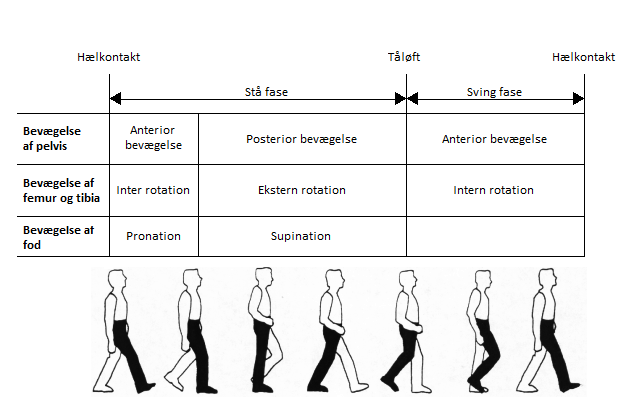
\includegraphics[width=0.8\textwidth]{figures/knaet}
\caption{Aktivering af hofte, knæet og ankel under gang \citep{orthopedics2016}.}
\label{fig:knaet}
\end{figure} 

\subsection{Knæets opbygning}
Knæleddet er et hængselled, hvilket medvirker til, at knæet kan rotere begrænset, fleksere og ekstensere. Knæet består af tre separate ledforbindelser. To, der er forbundet mellem femur og tibia, samt et mellem patella og femur, hvilket fremgår af \autoref{fig:knae_anatomi}. Ud over de tre separate ledforbindelser stabiliseres knæet af syv ledbånd. Ét af de syv ledbånd er patellarsenen, som er ansvarlig under extension af knæet. Derudover er der to ledbånd, som strækker sig mellem femur, tibia og fibia, hvilket er med til at styrke knæleddets overflade posteriort. Inde i ledkapslen befinder det forreste korsbånd (ACL) og det bagerste korsbånd (PCL), som har til opgave at fastgøre indre knoglefremspring af tibia til knoglefremspringet på femur. Korsbåndene har til opgave at begrænse anteriore og posteriore bevægelser af femur og er med til at opretholde retningen af knoglefremspringene. Det tibiale kollaterale ligament forstærker den mediale flade af knæleddet og det fibulære kollaterale ligament forstærker sidefladen. Disse ligamenter anvendes kun ved fuld ekstension \citep{martini2012}.

\begin{figure}[H]
\centering
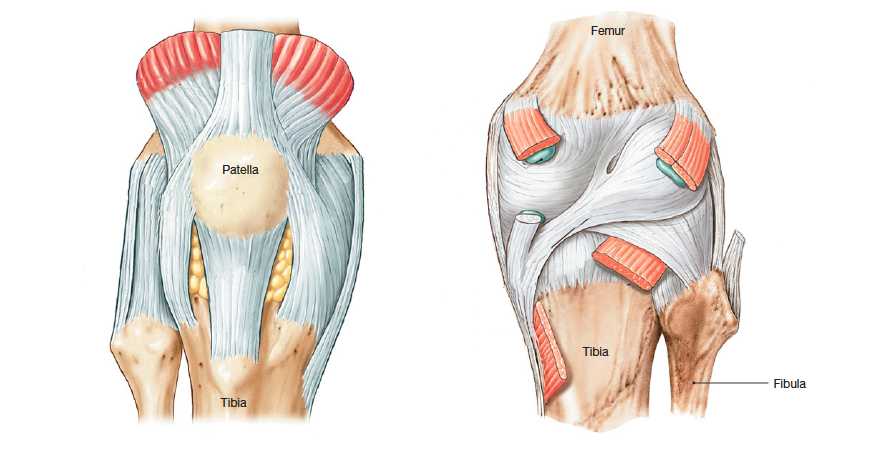
\includegraphics[width=0.8\textwidth]{figures/knae_anatomi}
\caption{Knæets anatomiske opbygning.}%\citep{kilde}
\label{fig:knae_anatomi}
\end{figure} 

\subsection{Knæets funktion}
Ved gang aktiveres quadricepsmusklerne, der sidder anteriort på femur, og hamstringmusklerne, der sidder poseriort på femur, hvilket fremgår af \autoref{fig:knae_anatomi}. Quadricepsmusklerne består af rectus femoris, vastus intermedius, vastus medialis og vastus lateralis. Hamstringmusklerne består af biceps femoris, semitendinosus og semimembranosus. Ved bevægelse foretager quadriceps- eller hamstringmusklerne ekstension eller fleksion, hvorved de fungerer som hinandens agonister eller antagonister under bevægelse \citep{martini2012}. 

Som tidligere nævnt anvendes hofte, knæ og ankler under gang. Udover disse led er også kropsposituren og sving af leddene afgørende for gangfunktionen. Det fremgår af \autoref{fig:knaet}, hvordan de forskellige led udfører fleksion, ekstension og ændres fra ekstension til neutral bevægelse under gang \citep{martini2012}.

\subsubsection{Knæets funktion under en squat-øvelse}
% mere om, at det kun er lårets muskulatur, der benyttes under squat
Knæets funktion for bøjningen af benet ses ved udførelse af en squat-øvelse. Under denne øvelse aktiveres quadricepsmusklerne ved $80 - 90^{\circ}$ fleksion og er herefter konsistent. Der ses en større aktivering af vastus intermedius, vastus medialis samt vastus lateris, da disse muskler er én ledmuskel, hvor rectus femoris er en to-ledsmuskel. Hamstringmusklerne aktiveres ved en $45^{\circ}$ fleksion \citep{schoenfeld2010}.
Ved udførelse af en squat-øvelse er det primært lårmusklerne, quadriceps- og hamstringsmusklerne, der aktiveres. 


 %der er forbundet mellem femur, tibia og patella. Knæet har fire ledbånd. To af disse er side-ligamenterne, der sidder omkring knæleddet. De resterende to er korsbåndene, der sidder på skrå inden i knæet.
%Knæet fire ledbånd sikrer stabilisering af knæet og sørger for at knoglerne bevæger sig rigtigt.  Det er knæleddet, der gør det muligt for kroppen at kunne udføre aktiviteter som at kunne gå, løbe, og eksempelvis squatte. Ved gang aktiveres både quadriceps musklerne (rectus femoris, vastus intermedius, vastus medialis, vastus lateralis) der sidder anteriort for låret samt hamstring musklerne (biceps femoris, semitendinosus, Semimembranosus), der sidder posteriort for låret og kontraherer med quadriceps musklerne. 

